\documentclass[11pt,a4paper]{article}
\usepackage[margin=22mm,top=19mm,bottom=20mm]{geometry}
\usepackage{amsmath,amssymb,graphicx,booktabs}
\usepackage{lmodern,microtype,xcolor}
\usepackage[hidelinks]{hyperref}

\definecolor{ink}{HTML}{172635}
\setlength{\parindent}{1em}
\setlength{\parskip}{0.18em}
\setlength{\emergencystretch}{2em}
\setlength{\textfloatsep}{13pt plus 3pt minus 2pt}
\setlength{\intextsep}{12pt plus 3pt minus 2pt}
\widowpenalty=10000
\clubpenalty=10000
\graphicspath{{figures/}}
\DeclareMathOperator{\Tr}{Tr}
\newcommand{\Wp}{\mathcal W_L}
\newcommand{\pp}[1]{\text{P3#1}}

\newcommand{\manuscripttitle}{Predictive Stopping and Memory-Assisted Adaptive Reconnection in Quantum Work Networks}
\hypersetup{pdftitle={\manuscripttitle},pdfauthor={Quantum Work Network project}}
\title{\vspace{-1.25em}\color{ink}\bfseries\manuscripttitle}
\author{Quantum Work Network project}
\date{Research Manuscript \textbullet\ First draft \textbullet\ 25 November 2026}

\begin{document}
\maketitle

\begin{abstract}
We study when to extract local work and when to reconnect the load of a finite quantum network. In drive-off, zero-dephasing simulations of a seven-qubit chain and a three-level load, the ergotropy rate is the load-energy current minus the passive-energy rate. A causal extrapolation of this rate located the first forecast within 0.10 model-time units of the best sampled extraction time on 15 of 33 trajectories. Repeated forecast-based extraction led a greedy hindsight comparator at time 50 on all four reference histories, and trailed it at time 540. A history-triggered switch to adaptive reconnection raised mean time-540 work from $50.212$ to $72.175$ in units of $10^{-6}$ on those histories, compared with $82.531$ for hindsight. A one-quadrature reconnection rule preserved performance on inherited states while using roughly half as many real-valued readouts, but on one separately prepared stress state it changed the sign of cumulative net work. Restoring both a switching-input and a phase condition recovered positive work there. The two decisions therefore rely on different information: changes in the load spectrum guide extraction timing, while both quadratures of terminal--load coherence can matter when accounting for reconnection and its downstream effects.
\end{abstract}

\section{Introduction}

A charged subsystem in a passive state gives up none of its bare energy under a local unitary. Ergotropy quantifies the portion of bare energy available to that operation for a general state \cite{pusz,allahverdyan}. Quantum-battery studies have examined how correlations constrain this portion and how the energetic cost of changing the battery--charger coupling enters a work cycle \cite{andolina,barra}. In a finite chain, the times of energy transfer, peak ergotropy and favorable switching work can differ. A repeated extractor must also operate on the state left by its previous decisions.

The Quantum Work Network project first studied drive, chain length, dephasing, and local work extraction, then followed saved states through storage and recovery \cite{project}. Here we synthesize the milestones around two control decisions: when to take work while connected, and when to restore the coupling after a disconnected wait. We compare the resulting policies on common elapsed clocks and use a matched-state intervention to trace a failure of a reduced-information controller. The accompanying supplement maps the earlier experiments, gives the rule parameters and identifies the data and audits behind the reported values.

\section{Physical Model}
\label{sec:model}

With $\hbar=1$, the drive-off Hamiltonian on $(\mathbb C^2)^{\otimes 7}\otimes\mathbb C^3$ is
\begin{align}
H(g) &= H_C + H_L + g(X+X^\dagger), \qquad X=\sigma_7^+ b,\\
H_C &= \omega\sum_{j=1}^{7}\sigma_j^+\sigma_j^-
   +\kappa\sum_{j=1}^{6}(\sigma_j^+\sigma_{j+1}^-+\sigma_j^-\sigma_{j+1}^+),\\
H_L &= \omega_L b^\dagger b, \qquad b=|0\rangle\langle1|+\sqrt{2}|1\rangle\langle2|.
\end{align}
The coherent continuations use $\omega=\omega_L=\kappa=1$ and $g=0.25$ when connected, with $g=0$ during a wait. Time and energy below are in model units. The reference preparation inherits a driven and dephased history. The continuations analyzed here evolve with zero drive and zero dephasing between operations.

Let $c=\Tr(\rho X)$, let $\rho_L=\Tr_C\rho$, and let $\lambda_k$ be the eigenvalues of $\rho_L$ in descending order. The energies $\epsilon_k$ of the load are indexed in ascending order. Then
\begin{equation}
 E_L=\Tr(\rho_L H_L), \qquad E_{\rm p}=\sum_k\epsilon_k\lambda_k, \qquad \Wp=E_L-E_{\rm p}.
\end{equation}
On connected segments, away from load eigenvalue degeneracies, the commutator equation gives
\begin{equation}
 J=\dot E_L=-2g\omega_L\operatorname{Im}c,\qquad
 D=\dot{\Wp}=J-\dot E_{\rm p},\qquad
 \dot E_{\rm p}=\sum_k\epsilon_k\langle v_k|\dot\rho_L|v_k\rangle,
 \label{eq:rate}
\end{equation}
where $|v_k\rangle$ belongs to $\lambda_k$. The terminal-qubit--load reduced state suffices to compute $\dot\rho_L$, because tracing out the chain removes the commutator with $H_C$. During a disconnected wait the load evolves under $H_L$, preserving $E_L$, $E_{\rm p}$, and $\Wp$, while $c$ can change as the joint state evolves.

\paragraph{Work accounting.}
For an instantaneous switch at fixed $\rho$, positive input is work supplied to the system. For $c_0$ just before disconnection and $c_\tau$ just before reconnection, total switching input is
\begin{equation}
 I_{\rm sw}=\underbrace{-2g\operatorname{Re}c_0}_{I_{\rm off}}
            +\underbrace{2g\operatorname{Re}c_\tau}_{I_{\rm on}}.
 \label{eq:switch}
\end{equation}
A load unitary passivates $\rho_L$ while the coupling is on. A deterministic eigenvector phase convention fixes the unitary. Its output is $W_{\rm pass}=\Wp-\Delta\langle g(X+X^\dagger)\rangle$, with the interaction change evaluated across the unitary. The trial's net output is $W_{\rm pass}-I_{\rm sw}$. If passivation is skipped, the two switching terms still count. At fixed $g$, between instantaneous operations the modeled total energy is conserved up to numerical propagation error.

\section{Methods}
\label{sec:methods}

\paragraph{Connected stopping.}
Policy A reads the terminal--load state every $h=0.02$. If $D_{i-1}>D_i>0$ and $\Wp(t_i)>10^{-12}$, it extrapolates a zero of the rate at a delay
\begin{equation}
 \widehat{\delta t}=h\frac{D_i}{D_{i-1}-D_i}.
 \label{eq:forecast}
\end{equation}
The first forecast with delay at most 0.10 and a valid target fixes the stopping time. The controller rounds to the nearest sampling point, at least one step forward, and otherwise uses the final available point. The decision to passivate uses a numerical work floor and, in the RK4 branches, an aligned-step error estimate. A trial lasts at most 18 time units including any wait. The single-extraction diagnostic evaluates each forecast against the best sampled work in its window. The repeated hindsight comparator E greedily searches its registered wait and extraction grid at each trial, including switching terms. E uses future states within that trial and represents a finite-grid comparator.

\paragraph{Memory and reconnection.}
The repeated adaptive policy begins with A and no waiting. At trial boundaries it compares the net recovery rate of accepted extractions in the last 24 units with its own early rate through time 32. The rate-only switch F1 enters waiting mode once a persistent slowdown qualifies. The phase-assisted switch F2-R also checks low load ergotropy and features of the terminal--load coherence and recent work. In waiting mode F2-R uses the phase-and-input rule RP before applying connected stopping A again. Here memory means stored observations and completed-work history in the classical controller.

Write $q_\tau=-\operatorname{Im}c_\tau$, with $q_0$ defined at the cut. The reduced rule P3 reconnects at the first waiting sample satisfying $q_\tau\ge\max(0.25|q_0|,10^{-11})$. RP instead uses a relative threshold $0.25|c_0|$, an amplitude floor $|c_\tau|\ge10^{-5}$, and both additional conditions
\begin{equation}
 I:\ \operatorname{Re}c_\tau-\operatorname{Re}c_0\le10^{-10},
 \qquad A_\phi:\ \arg c_\tau\in[-3\pi/4,-\pi/4].
 \label{eq:gates}
\end{equation}
The wait grid runs from 1 to 6 in steps of 0.2 for full-length windows. On reaching the cap the controller reconnects even when its conditions fail. $\pp{+I}$ and $\pp{+A}$ add one condition to P3, and $\pp{+IA}$ adds both. We use $A_\phi$ for the phase condition to distinguish it from connected stopping A. When $I$ passes, Eq.~\eqref{eq:switch} bounds total switching input by $2g\times10^{-10}$ for that candidate. The bound is conditional on the gate outcome at the executed time.

\paragraph{Comparisons and checks.}
Repeated policies start independently from the same saved state within each origin. Every operation carries the full resulting density matrix forward, including correlations. Four reference histories (S0, A04, B04, C04) share genealogy. The later reconnection comparisons branch from matched saved switch states and also include six separately prepared states (U01--U06) first used for the M29 transfer test. M30 reuses these states for its condition interventions. Coarse and half-step RK4 propagation use steps of 0.0025 and 0.00125, with separate control clocks for the main comparisons and aligned operations for numerical checks. Selected M30 branches also recompute the decisions with exact unitary propagation between operations.

\section{Results}
\label{sec:results}

\subsection{The ergotropy rate identifies near-term peaks}

M23 found higher best sampled single-window work after a variable wait than under continuous connection for S0 and S1, by 28.02\% and 68.22\% respectively. On S2 the best wait was zero. Initial current did not pick the best wait on any of those three origins. In M24, the signs of $J$ and $D$ disagreed at a median 48.6\% of above-floor observation points per trajectory. For example, ergotropy grew on the S0 trajectory with wait 4.90 at elapsed 15.08 while the load was exporting energy, because the passive energy fell faster than the load energy.

Across 33 trajectories, at least one rate forecast per trajectory flagged the best sampled work time within $\pm0.10$. The matching forecast occurred 0.08--0.10 before that time. The first forecast reached the same tolerance on 15 trajectories (Fig.~\ref{fig:stopping}a). The first current sign reversal did so on one. On nine additional saved starts under continuous connection, taking the first forecast delivered a mean 69.8\% of the corresponding same-wait best work and 59.7\% of the variable-wait hindsight value, with median duration 2.94 versus 8.45 for the variable-wait comparator. This is evidence for local timing and an early work-rate benefit, with later peaks remaining consequential.

\subsection{Repeated extraction changes the ranking over time}

In M25, at the same count of 30 extractions A recovered 57.5\% of E's mean work in 28.0\% of E's mean time. When M26 lifted the count cap, A led E on every reference history at elapsed times 50 and 100. The last crossover was between 109.65 and 132.41 across the four origins. From time 150 through time 540 E led A on all four. At 540 the mean work was $50.212\times10^{-6}$ for A and $82.531\times10^{-6}$ for E (Fig.~\ref{fig:stopping}b). The run end is the chosen observation horizon.

The M27 controller retained A's early output because its first mode switch came after time 50 on each origin. At time 540, F1 reached $70.599\times10^{-6}$ and the phase-assisted policy reached $72.175\times10^{-6}$, or 87.45\% of E's mean endpoint work. M28 stabilized the phase-assisted switch by applying the floor $D>10^{-12}$ to the positive-rate clause of its mode-switch gate. For C04, this removed a coarse/half timing divergence arising from machine-scale rates after passivation. The corrected F2-R retained the coarse mean reported above.

\begin{figure}[!htbp]
  \centering
  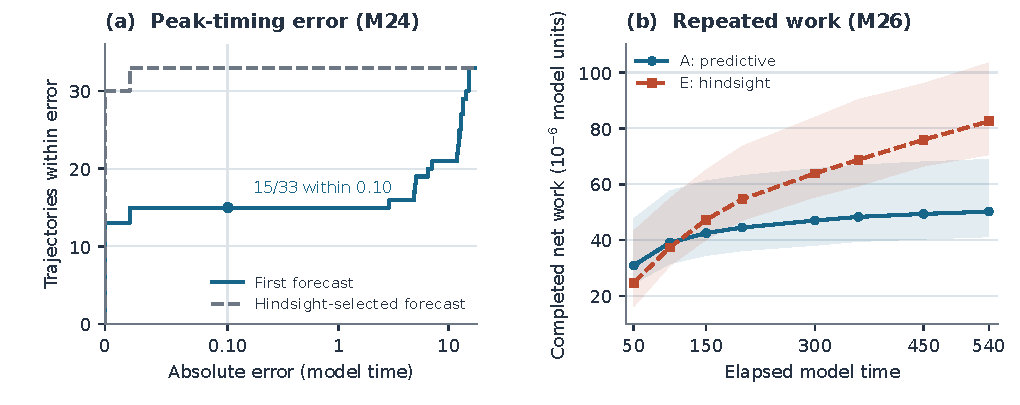
\includegraphics[width=0.97\linewidth]{predictive_stopping.pdf}
  \caption{Forecast accuracy and the elapsed-time comparison for repeated control. (a) The first forecast and a retrospectively matched forecast are each compared with the best sampled work time at the same wait. (b) Completed-trial work means and min--max ranges across the four reference histories. Sources are M24 and M26.}
  \label{fig:stopping}
\end{figure}

\subsection{Reduced reconnection information transfers unevenly}

In the M28 post-switch branches from matched F2-R anchors, RP recovered mean work $36.120\times10^{-6}$ by time 540. Fixed wait 3 and the history-based arm selector RH gave $33.850$ and $34.596$ in the same units. Some individual origins favored fixed or empirical waits (Fig.~\ref{fig:adaptive}a). In M29, the imaginary-only P3 policy retained a ratio of group mean work of 102.31\% and 103.36\% relative to RP in the F2-R and F1 anchor groups. Its lowest individual ratios there were 94.96\% and 98.96\%. For the F2-R anchors, P3 used an average of 823.5 real-valued coherence components per run, compared with 1,636.0 for RP. The number of sample times increased slightly (Fig.~\ref{fig:adaptive}b).

Across U01--U06, P3 retained 78.75\% of RP's group mean, with five of six states retaining at least 90\% individually. The U05 endpoint changed from $+1292.742\times10^{-6}$ under RP to $-790.453\times10^{-6}$ under P3, whereas U06 reached 111.16\% of RP. These pooled ratios weight states by their work scale and the six origins span a wide range of work. On the reference histories from their original initial conditions, a rate-only switch followed by P3 (M3) gave mean $74.064\times10^{-6}$ at time 540. This whole-history result and the matched-anchor comparisons answer different control questions.

\begin{figure}[!htbp]
  \centering
  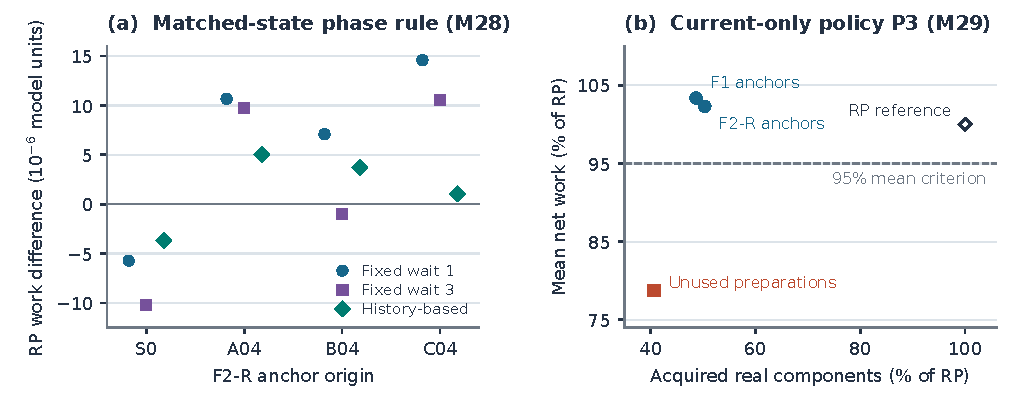
\includegraphics[width=0.97\linewidth]{adaptive_reconnection.pdf}
  \caption{Matched-state reconnection comparisons and the information--work tradeoff. (a) Time-540 work differences between RP and fixed or history-based waiting on shared F2-R anchors. (b) Ratios of P3 to RP for group means of work and real-valued parts of $c$ acquired for reconnection. The dashed line is the 95\% group-mean work criterion. Sources are M28 and M29.}
  \label{fig:adaptive}
\end{figure}

\subsection{A matched-state intervention links losses to switching input}

In the sixth U05 trial all eight rules cut from the same state at elapsed time 44.44. P3 and P1 selected wait 2.4, where both $I$ and $A_\phi$ fail. Each restored condition was sufficient to reject that point and all six restored branches waited to the forced cap of 6, where the full gate need not be satisfied. Switch-on input changed from $+328.498$ to $-186.267$, the common switch-off output was $29.816$, and passivation changed from zero to $8.512$, all in units of $10^{-6}$. The net trial output moved from $-298.682$ to $+224.595$ (Fig.~\ref{fig:u05}a). The switch-on change accounts for $514.765$ of the $523.277$ improvement.

After this common intervention, subsequent trajectories differ. At elapsed time 540, U05 work was $-790.453$, $+435.939$, $-710.350$, and $+1816.703$ in units of $10^{-6}$ for P3, $\pp{+I}$, $\pp{+A}$, and $\pp{+IA}$, respectively. RP gave $+1292.742$ (Fig.~\ref{fig:u05}b). The effect of adding both conditions minus the sum of the separate effects was $-523.277$ for the single common trial and $+1300.661$ at the endpoint. The endpoint contrast summarizes entire policy trajectories, including different later states and choices. $\pp{+IA}$ was the only intervention to satisfy both the 95\% group-mean and 90\% per-state retention criteria relative to RP in all three evaluated groups. It read both quadratures and omitted the amplitude calculation used by RP.

At the level of the controls, all 112 RK4 coarse/half pairs and all 16 U05/U06 coarse/exact-online pairs agreed on discrete actions, with maximum endpoint differences $8.33\times10^{-12}$ and $8.87\times10^{-12}$, respectively. In a separate fixed-operation check, continuous exact propagation exceeded earlier state or energy tolerances on 20 of 32 stress-state branches. The maximum energy deviation was $1.076\times10^{-11}$ and the maximum saved density-element deviation was $8.005\times10^{-10}$. These deviations are recorded in the original audits alongside the agreement of the online decisions.

\begin{figure}[!htbp]
  \centering
  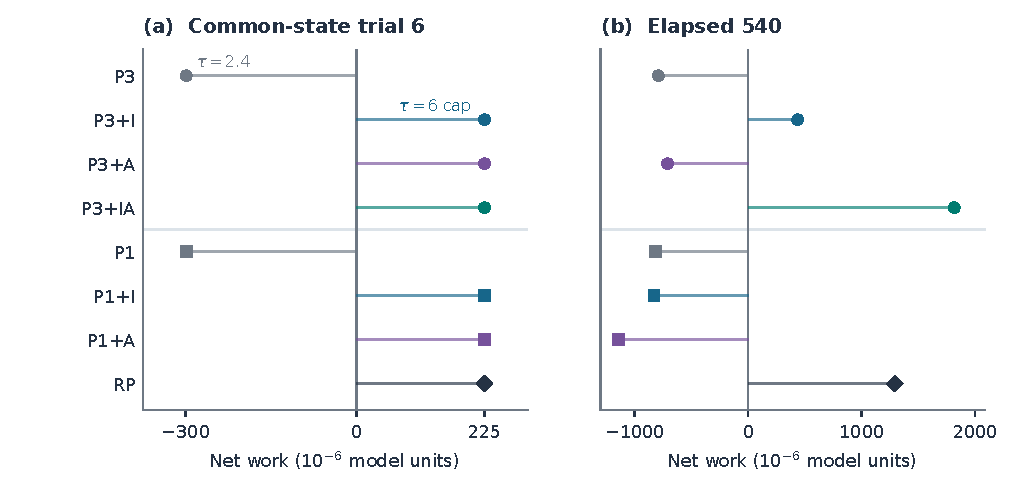
\includegraphics[width=0.97\linewidth]{u05_reconnection.pdf}
  \caption{U05 reconnection intervention at the common sixth cut. (a) Net work of the first trial after forking at elapsed 44.44. (b) Cumulative event-clock work from preparation to elapsed 540. The panels use different scales. Source is M30.}
  \label{fig:u05}
\end{figure}

\section{Discussion}

Equations~\eqref{eq:rate} and \eqref{eq:switch} explain why the two stages reward different observables. During connected evolution the load spectrum can absorb or release passive energy at a rate comparable to the incoming current. During decoupled waiting, $q_\tau$ indicates the prospective current immediately after reconnection. The change in the real quadrature determines the cost of the two switches. A current gate alone leaves that cost unidentified. A phase window couples restrictions on the two quadratures, and the input gate compares the real component with its own pre-cut value.

U05 shows how this distinction matters for net work. Over its full trajectory, the P3 and $\pp{+IA}$ passivation outputs are close ($71.193$ versus $70.750$, in units of $10^{-6}$), while their switching inputs have different signs ($+861.646$ versus $-1745.953$). In the common sixth trial the added conditions worked by rejecting an early switch. Later divergences show that a veto's single-trial effect is insufficient to determine its cumulative effect. The result extends the accounting perspective used in cyclic battery models \cite{barra} to a finite-time, history-dependent policy comparison on this network.

\section{Limitations}

The controller reads exact model expectations and reduced states. The work ledger includes modeled switching and passivation, with measurement, estimation, feedback, and pulse implementation outside the simulation budget. The reported component counts measure information access in the simulation. Connecting them to an apparatus would require a measurement model with precision, sampling, backaction, and control overhead.

The main experiments use one finite network, one connected coupling, and noiseless post-preparation dynamics. The four reference histories and the eight inherited switch anchors share ancestry. The six preparation variants span a wider range, yet they are a small designed set and were reused in M30 for intervention analysis. The aggregate ratios characterize those groups. The finite-grid hindsight policy is greedy per trial, and all results are bounded by the chosen windows and elapsed horizon. The tested thresholds and the common-state intervention establish behavior for the modeled cases. A broader literature review and independent tests across models and preparations would be needed to establish novelty and generality.

\section{Conclusion}

An ergotropy-rate forecast provided early extraction times and improved early repeated recovery on the four reference histories. History-triggered reconnection recovered part of the longer-horizon gap to a greedy hindsight policy. The stress-state intervention identified a limit of reducing reconnection to one coherence component: prospective current can favor a switch that incurs a larger energetic cost than the rest of the trial recovers. Preserving an explicit signed work ledger and separating local forecasts from long-horizon comparisons made that failure and its timing mechanism visible.

\section*{Data and code availability}

The companion \texttt{supplementary.md} records the milestone sources, data files, numerical checks, and figure build commands. Figures summarize already recorded numerical output. The public project record provides the earlier history \cite{project}.

\begin{thebibliography}{9}
\bibitem{pusz} W. Pusz and S. L. Woronowicz, ``Passive states and KMS states for general quantum systems,'' \emph{Commun. Math. Phys.} \textbf{58}, 273--290 (1978). \href{https://doi.org/10.1007/BF01614224}{doi:10.1007/BF01614224}.
\bibitem{allahverdyan} A. E. Allahverdyan, R. Balian, and Th. M. Nieuwenhuizen, ``Maximal work extraction from finite quantum systems,'' \emph{Europhys. Lett.} \textbf{67}, 565--571 (2004). \href{https://doi.org/10.1209/epl/i2004-10101-2}{doi:10.1209/epl/i2004-10101-2}.
\bibitem{andolina} G. M. Andolina, M. Keck, A. Mari, M. Campisi, V. Giovannetti, and M. Polini, ``Extractable work, the role of correlations, and asymptotic freedom in quantum batteries,'' \emph{Phys. Rev. Lett.} \textbf{122}, 047702 (2019). \href{https://doi.org/10.1103/PhysRevLett.122.047702}{doi:10.1103/PhysRevLett.122.047702}.
\bibitem{barra} F. Barra, K. V. Hovhannisyan, and A. Imparato, ``Quantum batteries at the verge of a phase transition,'' \emph{New J. Phys.} \textbf{24}, 015003 (2022). \href{https://doi.org/10.1088/1367-2630/ac43ed}{doi:10.1088/1367-2630/ac43ed}.
\bibitem{project} Quantum Work Network project, \href{https://github.com/Riku-Tono/quantum-work-network/tree/ca760bb64584bb84ed8c917010c60faa0c092da0}{public milestone record at revision \texttt{ca760bb}}.
\end{thebibliography}

\end{document}
